\chapter{前端重构与界面修缮}

\section{构建基线修复}

前端首先恢复 TypeScript 构建基线，主要处理：

\begin{itemize}
  \item TanStack Table \code{ColumnMeta.title} 类型补充。
  \item 表单 resolver 类型兼容。
  \item 数字和字符串筛选值统一。
  \item 未使用模板代码对构建的阻塞。
\end{itemize}

最终 \code{npm run build} 已通过。

\section{模板残留清理}

原项目保留了模板后台中的默认用户、示例团队和英文文案。重构后：

\begin{itemize}
  \item 侧栏文案改为 BikeHub 业务模块。
  \item 登录页改为中文业务文案。
  \item 默认用户和团队信息替换为运营调度平台信息。
  \item 主题设置从浮动抽屉融入正式设置页面。
\end{itemize}

\section{运营中台化视觉}

前端视觉调整遵循“运营中台”原则：克制背景、清晰侧栏、紧凑头部、统一表格和卡片间距。重点优化页面包括：

\begin{itemize}
  \item 仪表盘：增加任务统计、站点排行、预测需求和地图视图。
  \item 站点管理：统一搜索、筛选、列视图和表格布局。
  \item 调度管理：展示任务状态、优先级和操作入口。
  \item 需求管理：提供实时需求和预测需求两个视图。
  \item 设置页面：集中管理个人资料、主题、侧栏、布局和阅读方向。
\end{itemize}

\begin{figure}[htbp]
  \centering
  \begin{minipage}{0.48\textwidth}
    \centering
    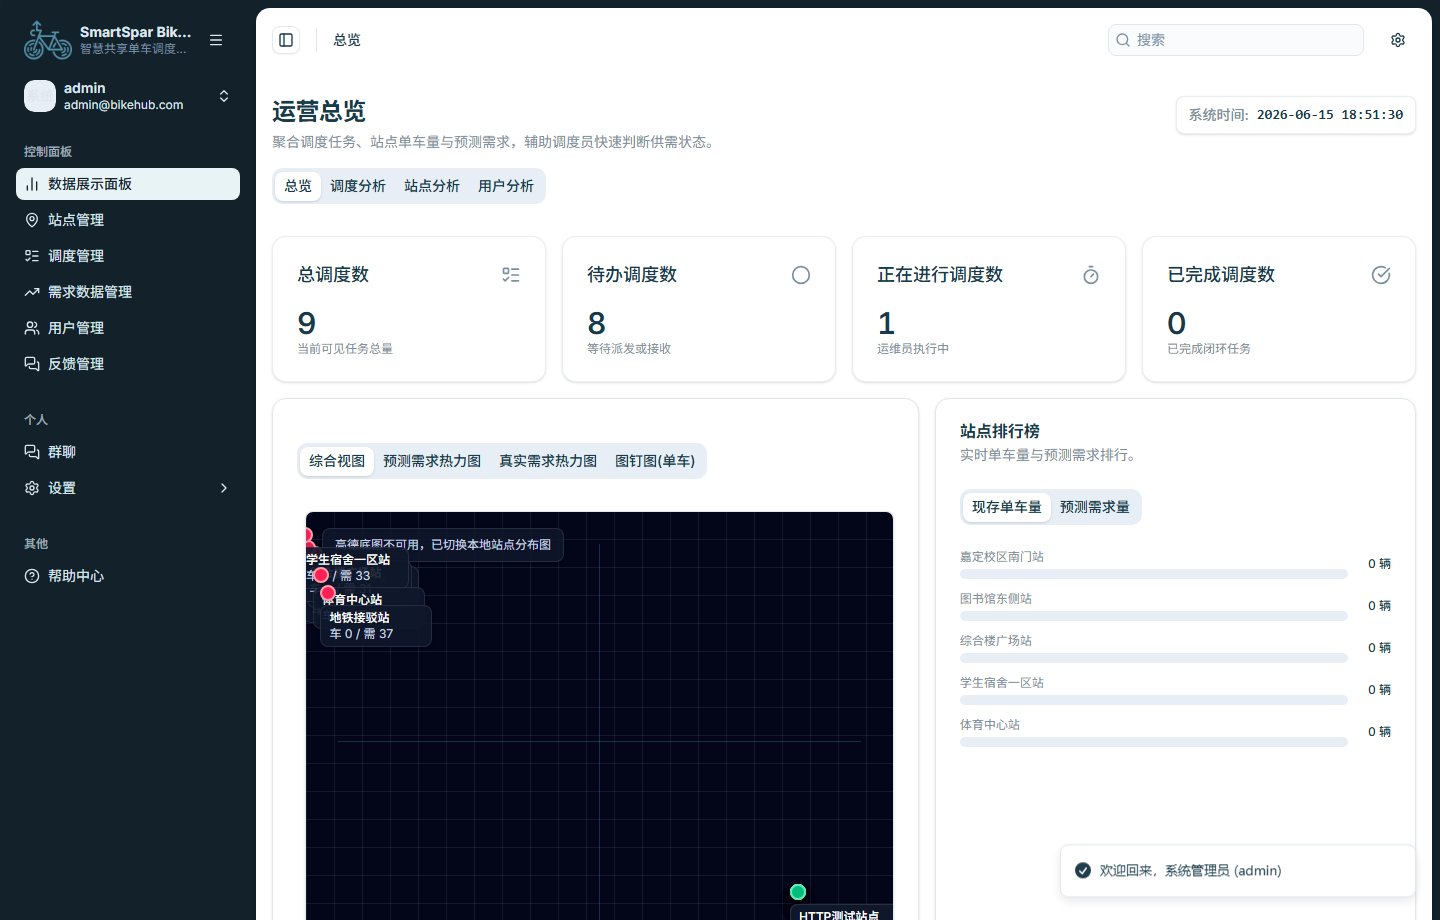
\includegraphics[width=\linewidth]{figures/evidence/ui_02_dashboard.png}
    \caption*{(a) 运营总览：任务统计、站点排行与地图视图}
  \end{minipage}\hfill
  \begin{minipage}{0.48\textwidth}
    \centering
    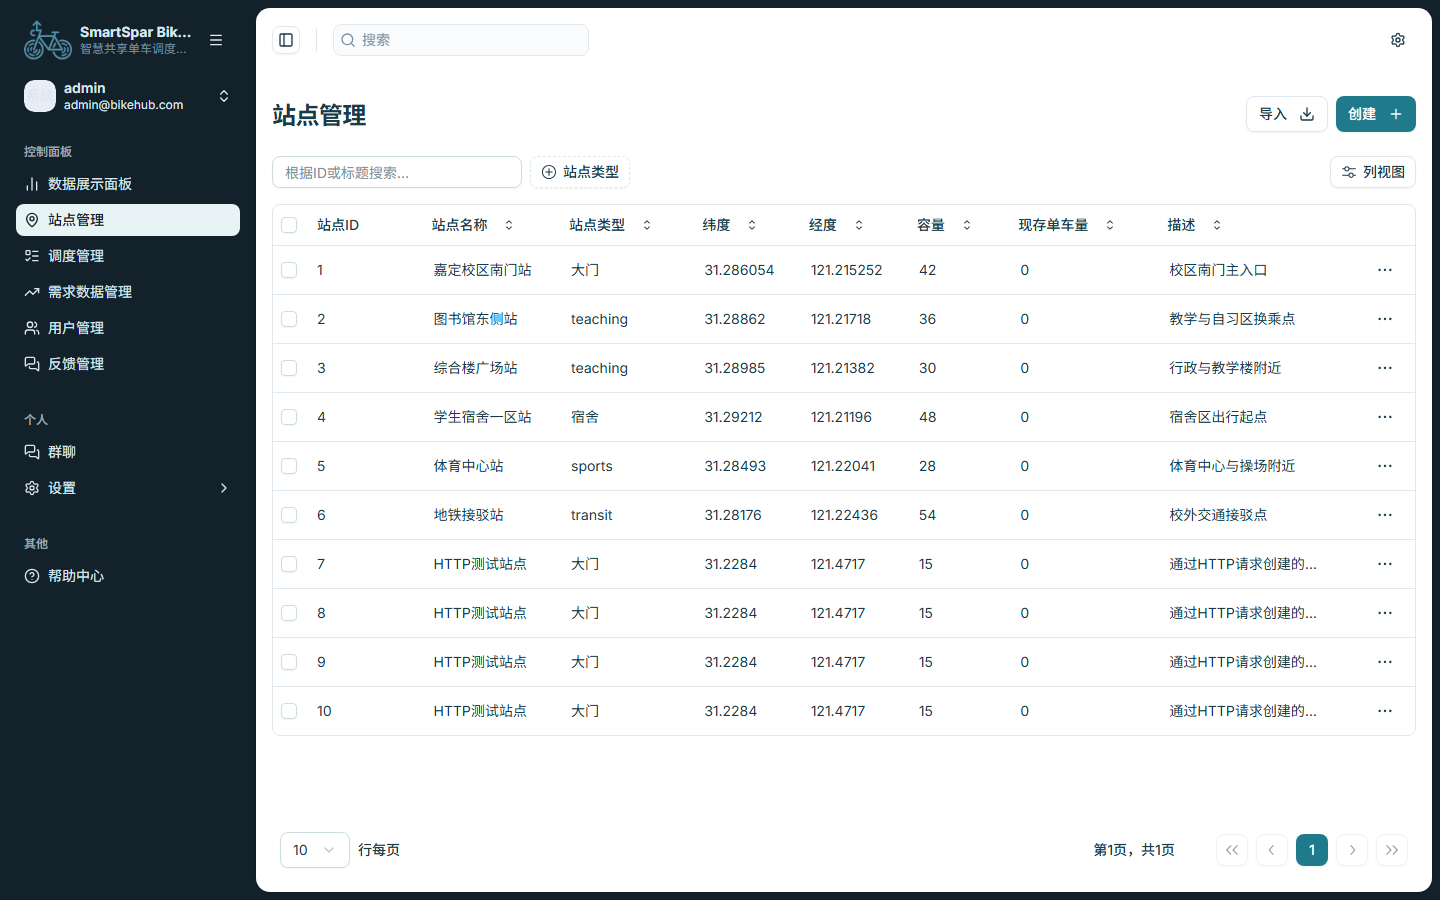
\includegraphics[width=\linewidth]{figures/evidence/ui_03_stations.png}
    \caption*{(b) 站点管理：搜索、导入、创建与表格布局}
  \end{minipage}

  \vspace{0.6em}

  \begin{minipage}{0.48\textwidth}
    \centering
    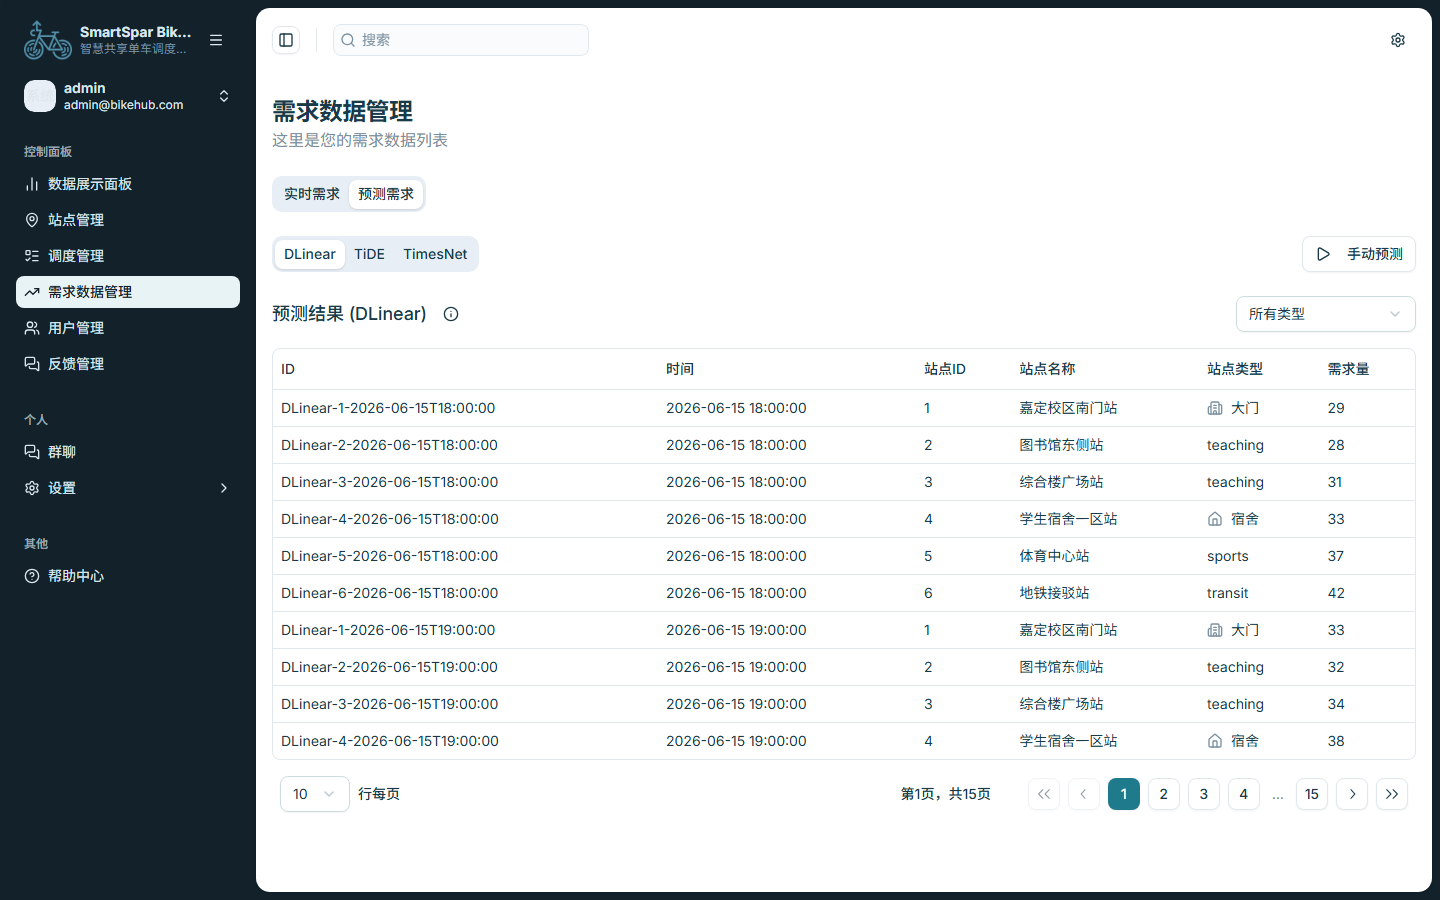
\includegraphics[width=\linewidth]{figures/evidence/ui_05_demand_prediction.png}
    \caption*{(c) 需求预测：DLinear future 数据展示}
  \end{minipage}\hfill
  \begin{minipage}{0.48\textwidth}
    \centering
    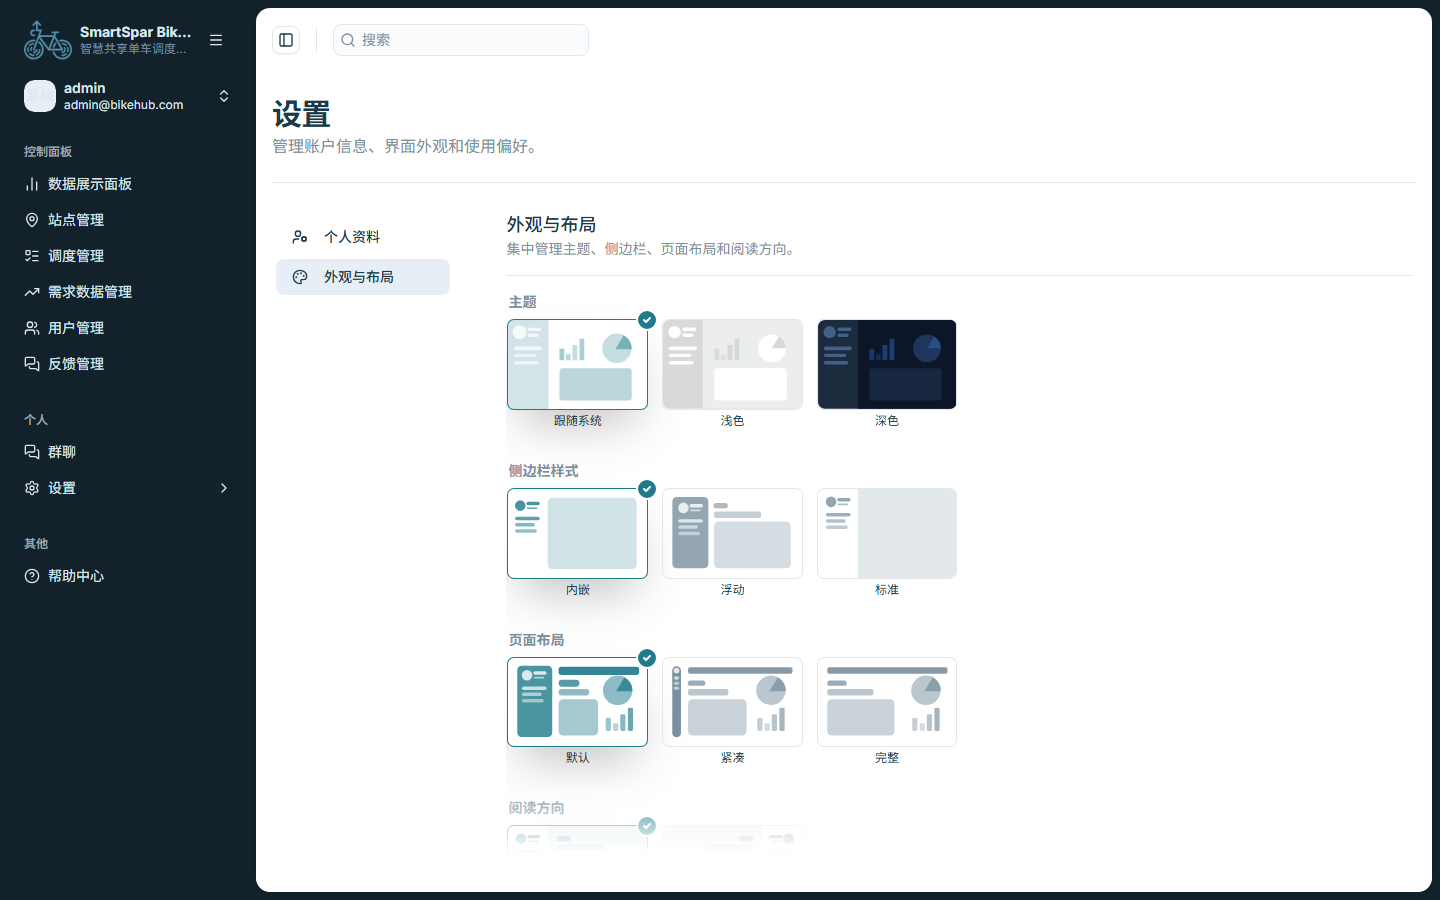
\includegraphics[width=\linewidth]{figures/evidence/ui_06_settings_appearance.png}
    \caption*{(d) 设置页面：外观、侧栏、布局和阅读方向}
  \end{minipage}
  \caption{前端核心页面重构效果截图}
\end{figure}

\section{地图体验优化}

仪表盘地图使用高德地图。考虑到本地网络、Key 或安全码可能不可用，重构中增加了 fallback：

\begin{itemize}
  \item 高德底图可用时展示真实地图。
  \item 高德底图不可用时切换为本地站点分布图。
  \item 地图容器采用稳定高度和边框，避免空白区域影响页面观感。
\end{itemize}
